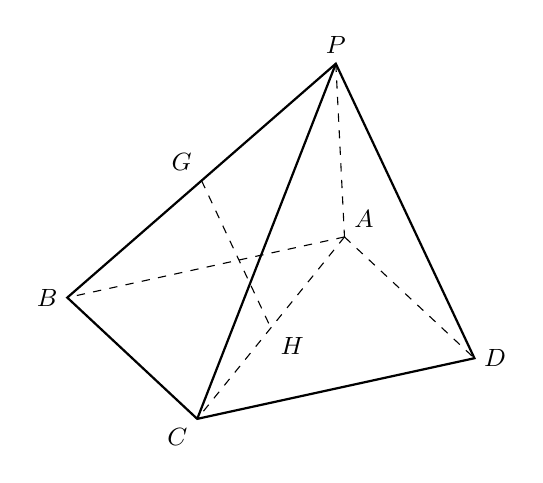
\begin{tikzpicture}[>=latex, font=\small, scale=1.1]
  % 顶点坐标
  \coordinate (P) at (1.1, 2.3);
  \coordinate (A) at (1.2, 0.3);
  \coordinate (B) at (-2.0, -0.4);
  \coordinate (C) at (-0.5, -1.8);
  \coordinate (D) at (2.7, -1.1);

  % 中点坐标
  \coordinate (G) at (-0.45, 0.95);
  \coordinate (H) at (0.35, -0.75);

  % 虚线不可见边与内部线段
  \draw[dashed, thin] (P) -- (A);
  \draw[dashed, thin] (A) -- (B);
  \draw[dashed, thin] (A) -- (D);
  \draw[dashed, thin] (A) -- (C);
  \draw[dashed, thin] (G) -- (H);

  % 实线可见外轮廓与面边界
  \draw[thick] (P) -- (B) -- (C) -- (D) -- cycle;
  \draw[thick] (P) -- (C);

  % 顶点标记
  \node[above] at (P) {$P$};
  \node[above right] at (A) {$A$};
  \node[left] at (B) {$B$};
  \node[below left] at (C) {$C$};
  \node[right] at (D) {$D$};
  \node[above left] at (G) {$G$};
  \node[below right] at (H) {$H$};
\end{tikzpicture}
